\chapter{Technische Umsetzung}
\section{Anforderungen und Rahmenbedingungen}
\section{Programmatische Konfiguration in Moodle}
\section{Gestaltung der Zertifizierung}



% In Unternehmen werden Schnittstellen zwischen verschiedenen Projekten durch den Einsatz eines Projektportfolio-Managements überwacht und dirigiert.
% \footcite[Vgl.][S. 356 f.]{bilginHandlingProjectDependencies2017}
% Die Einflüsse der anderen Projekte werden offensichtlich, wenn die Abhängigkeiten, welche durch die Aufgabengebiete definiert sind,
% dargestellt werden. Diese Einflüsse können, wie im Kapitel Risiko erläutert, überaus Einfluss auf die Qualität und die Zeitplanung des Projektes haben.
% Um diesen Einfluss darstellen zu können, wird die Kontextebene des C4-Modells verwendet, um einen Überblick über die Schnittstellen zu erhalten.
% \begin{figure}[H]
%     \centering
%     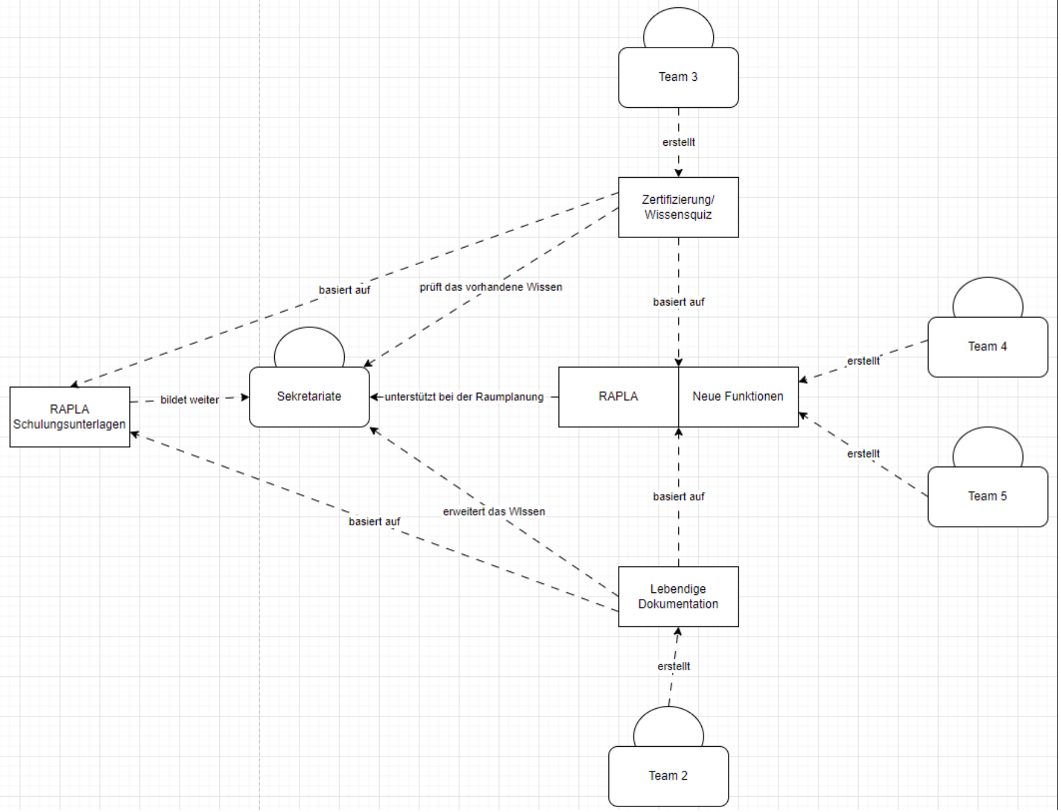
\includegraphics[width=1\linewidth]{graphics/rapla_model.png}
%     \caption{Schnittstellen im vorliegenden Projekt.}\label{abb:zeitplanung}
% \end{figure}
% Wie an diesem Modell sichtbar, gibt es für dieses Projekt (Team drei) 
% hauptsächlich eine direkte Abhängigkeit zu den Teams vier und fünf, da die
% Zertifizierung bestenfalls neue Funktionen von \ac{RAPLA} berücksichtigt und prüft. Allerdings
% gibt es auch eine indirekte Schnittstelle zu Team zwei, da diese ihre lebendige Dokumentation
% auf den gleichen Quellen (\ac{RAPLA} und \ac{RAPLA} Schulungsunterlagen) aufbaut. Durch klare Absprache
% können Mehrarbeit und Dopplungen vermieden werden.

% Aufbauend auf diesen Schnittstellen wird für die Zukunft folgende Zusammenarbeits-Maxime definiert: 
% Die Entwicklung der Teams vier und fünf werden verfolgt und es werden bereits vor deren Fertigstellung Platzhalter
% in der Zertifizierung geschaffen, um die Entwicklungen direkt nach ihrer Fertigstellung gegebenenfalls in die
% Zertifizierung aufnehmen zu können (soweit sie auch von den Schulungsunterlagen aufgenommen werden).
% Während sich die Interaktion mit den Teams Teams vier und fünf eher auf die zweite Hälfte des Projektes
% beziehen wird, besteht das Absprache-Potenzial mit Team zwei von Beginn an. Daher werden regelmäßige Absprachen
% sowie ein Austausch von Informationen geplant. Zusätzlich werden außerplanmäßige Treffen bei der Koordination
% von bestimmten Arbeitspaketen oder zu besonderen Anlässen wie Rücksprachen mit den Stakeholdern stattfinden.

Die Umsetzung des Projektes des Projektes erfolgt in zwei voneinander getrennten, eigens bereitsgestellten RAPLA-Instanzen